% !TEX root = ../main.tex
\section{Study Results}
\begin{frame}{}
    \centering \Huge{\ef{Study Results}}

    \vspace{9pt}

    \small{\textit{
        All plots in this section are from RG-F run 12016 w/ acceptance correction \textsuperscript{\textcolor{efd_purple}{\ref{20.10a::q2}} - \textcolor{efd_purple}{\ref{20.10h::phipq_pi-}}}.
    }}

    \small{\textit{
        \ef{Target:} H2 gas.
        \ef{Beam:} 250 nA, 10.4 GeV.
        \ef{Solenoid:} -0.75 (inbending).
        \ef{Torus:} -1.
    }}
\end{frame}

\subsection{Phase Space Study}
% !TEX root = ../main.tex
% --+ 12.11 SUMMARY +-----------------------------------------------------------
\begin{frame}{Phase Space Study}
    \label{12.11::summary}

    To select the region where to place the target, a phase space study was conducted.

    \vspace{12pt}
    \begin{itemize}
        \item
            The RG-F target gas region (\ef{$-30 < v_z < 20$} \textcolor{efd_green}{cm}) was divided into ten 5 cm bins.

        \vspace{6pt}
        \item
            The phase space of each relevant kinematic variable (\ef{$Q^2$}, \ef{$\nu$}, \ef{$z_h$}, \ef{$p_T^2$}, \ef{$\phi_{PQ}$}) was analysed for each bin.

        \vspace{6pt}
        \item
            The objective is to \ef{find a region that maximises each phase space}.

        \vspace{6pt}
        \item
            The error bars shown are the quadratic addition of the measurement and acceptance errors\appref{20.09::study_error_estimation}.
    \end{itemize}
\end{frame}

% --+ 12.12 Q2 +----------------------------------------------------------------
\begin{frame}{Phase Space Study: $Q^2$}
    \label{12.12::q2}

    \begin{columns}[onlytextwidth,T]

    \begin{column}{.80\linewidth}
        \vspace{-15pt}
        \begin{center}
            \begin{figure}[t]
                \centering{
                    \fbox{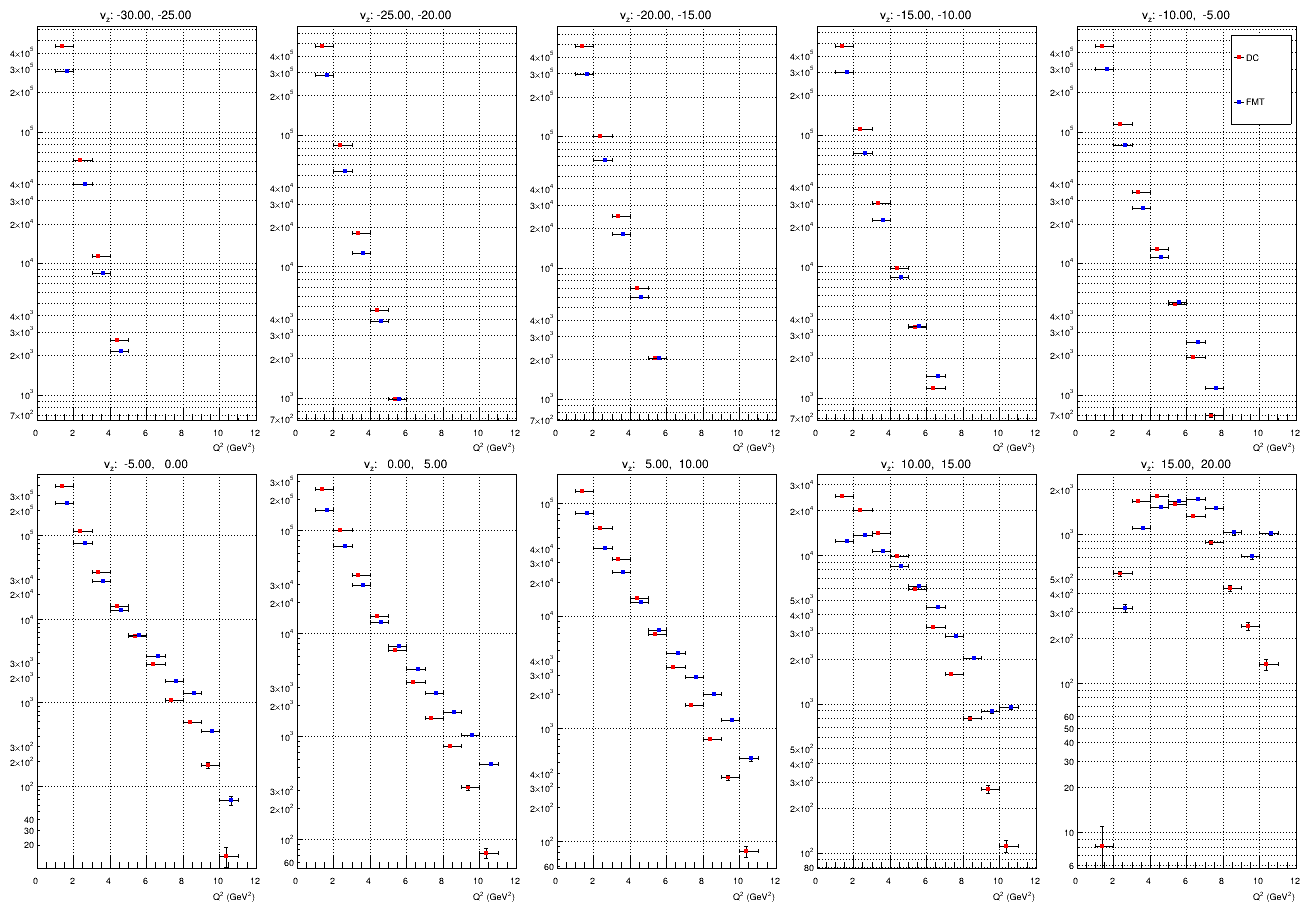
\includegraphics[width=\textwidth]{12q2.png}}
                }
            \end{figure}
        \end{center}
    \end{column}

    \begin{column}{.18\linewidth}
        \small{\ef{$v_z < -5$} \textcolor{efd_green}{cm}: \\ higher end of the phase space is limited.}

        \vspace{12pt}

        \small{\ef{$v_z > 15$} \textcolor{efd_green}{cm}: \\ $Q^2$ has an unusual shape.}

        \vspace{12pt}

        \small{\ef{Both effects are attributed to the FMT acceptance region.}}

        \vspace{18pt}

        \begin{flushright}
            \tiny{\textit{
                Bin markers are slightly shifted in $x$ for legibility.
                Uncorrected bins can be seen in Slide \textcolor{efd_purple}{\ref{20.10a::q2}}.
            }}
        \end{flushright}
    \end{column}

    \end{columns}
\end{frame}

% --+ 12.13 NU +----------------------------------------------------------------
\begin{frame}{Phase Space Study: $\nu$}
    \label{12.13::nu}

    \begin{columns}[onlytextwidth,T]

    \begin{column}{.48\linewidth}
        \vspace{-15pt}
        \begin{center}
            \begin{figure}[t]
                \centering{
                    \fbox{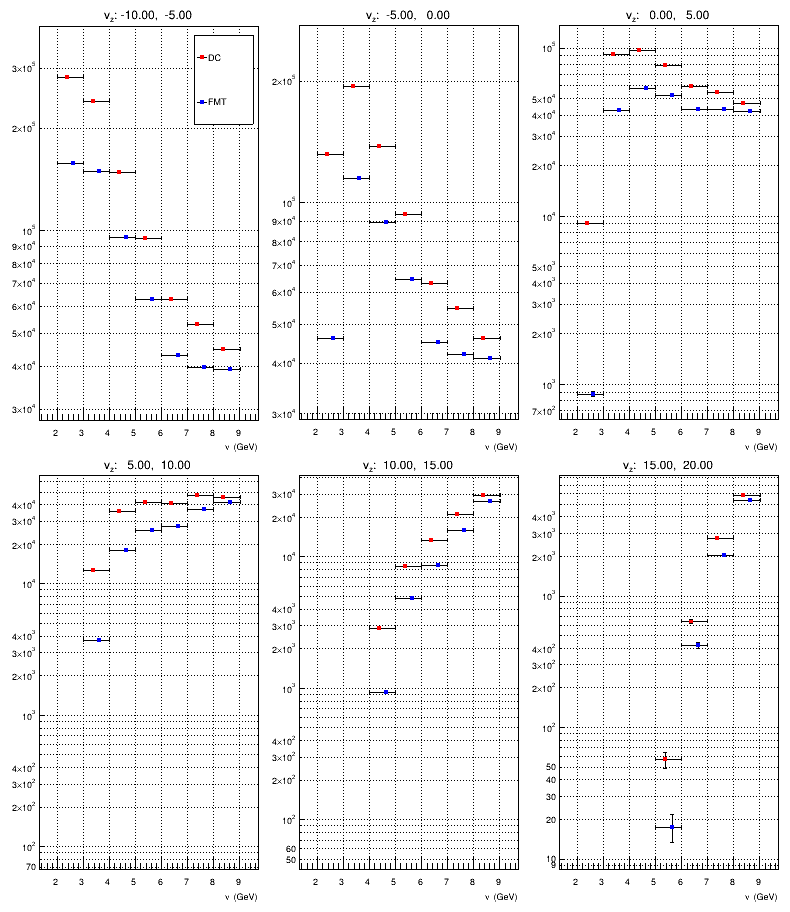
\includegraphics[width=\textwidth]{13nu.png}}
                }
            \end{figure}
        \end{center}
    \end{column}

    \begin{column}{.50\linewidth}
        \begin{itemize}
            \item
                \ef{$\nu$} has no direct correlation with the scattering angle \ef{$\theta_C$}.

            \vspace{12pt}
            \item
                \ef{$v_z > 10$} \textcolor{efd_green}{cm}: The lower end of $\nu$'s phase space is lost.

            \vspace{12pt}
            \item
                Based on the behaviour of both $e^-$ variables, $v_z$ will be restricted to \textcolor{efd_green}{$-5 \text{ cm} < v_z < 10 \text{ cm}$}.
        \end{itemize}

        \vspace{69pt}

        \begin{flushright}
            \tiny{\textit{Bin markers are slightly shifted in $x$ for legibility.}}

            \tiny{\textit{
                Other bins can be seen in Slide \textcolor{efd_purple}{\ref{20.11b::nu}}.
                Uncorrected bins in Slide \textcolor{efd_purple}{\ref{20.10b::nu}}.
            }}
        \end{flushright}
    \end{column}

    \end{columns}
\end{frame}

% --+ 12.14 ZH +----------------------------------------------------------------
\begin{frame}{Phase Space Study: $z_h$}
    \label{12.14::zh}

    \begin{columns}[onlytextwidth,T]

    \begin{column}{.44\linewidth}
        \vspace{-15pt}
        \begin{center}
            \begin{figure}[t]
                \centering{
                    \fbox{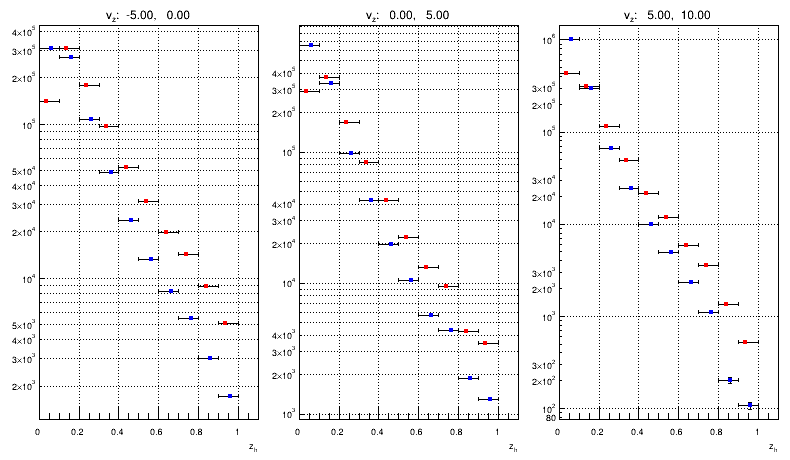
\includegraphics[width=\textwidth]{14zh_pi-.png}}
                }
                \scriptsize{\textit{$z_h$ distributions for \ef{$\pi^-$}.}}
            \end{figure}

            \vspace{-15pt}
            \begin{figure}[t]
                \centering{
                    \fbox{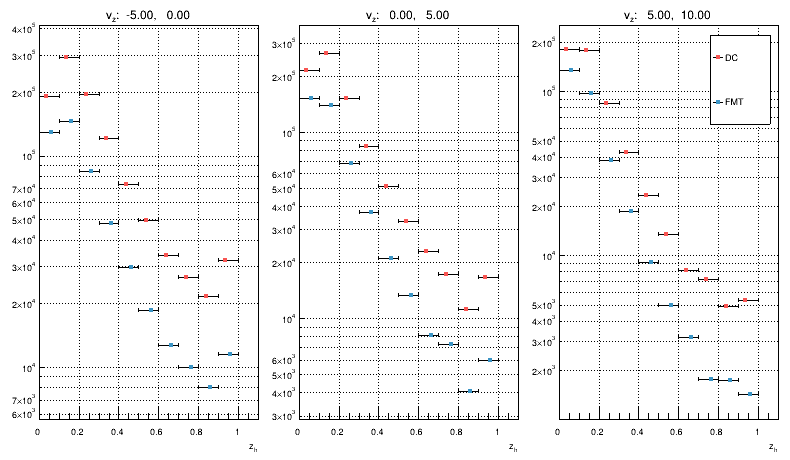
\includegraphics[width=\textwidth]{14zh_pi+.png}}
                }
                \scriptsize{\textit{$z_h$ distributions for \ef{$\pi^+$}.}}
            \end{figure}
        \end{center}
    \end{column}

    \begin{column}{.54\linewidth}
        \begin{itemize}
            \item
                Being hadronic variables, the \ef{$\theta$} dependence of $z_h$, $p_T^2$, and $\theta_{PQ}$ is not easily described.

            \vspace{12pt}
            \item
                \ef{No new restrictions on $v_z$ are derived from the $z_h$ distributions.}
        \end{itemize}

        \vspace{111pt}

        \begin{flushright}
            \tiny{\textit{Bin markers are slightly shifted in $x$ for legibility.}}

            \tiny{\textit{
                Other bins can be seen in Slides \textcolor{efd_purple}{\ref{20.11c::zh_pi+}} and \textcolor{efd_purple}{\ref{20.11d::zh_pi-}}.
                Uncorrected bins in Slides \textcolor{efd_purple}{\ref{20.10c::zh_pi+}} and \textcolor{efd_purple}{\ref{20.10d::zh_pi-}}.
            }}
        \end{flushright}
    \end{column}

    \end{columns}
\end{frame}

% --+ 12.15 PT2 +---------------------------------------------------------------
\begin{frame}{Phase Space Study: $p_T^2$}
    \label{12.15::pt2}

    \begin{columns}[onlytextwidth,T]

    \begin{column}{.44\linewidth}
        \vspace{-15pt}
        \begin{center}
            \begin{figure}[t]
                \centering{
                    \fbox{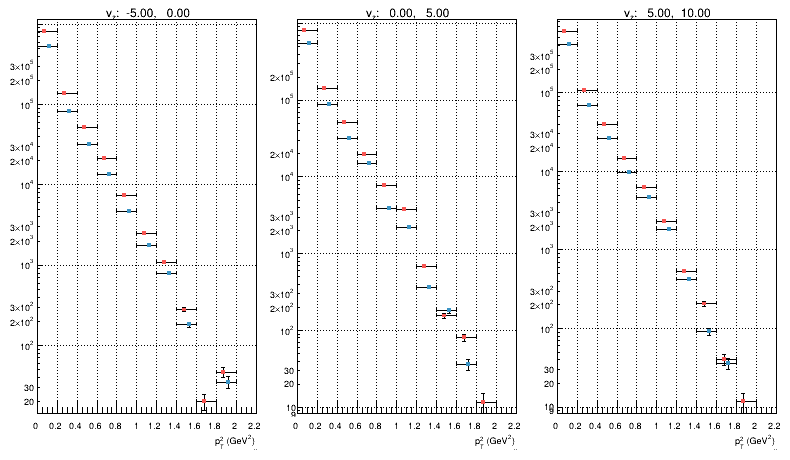
\includegraphics[width=\textwidth]{15pt2_pi-.png}}
                }
                \scriptsize{\textit{$p_T^2$ distributions for \ef{$\pi^-$}.}}
            \end{figure}

            \vspace{-15pt}
            \begin{figure}[t]
                \centering{
                    \fbox{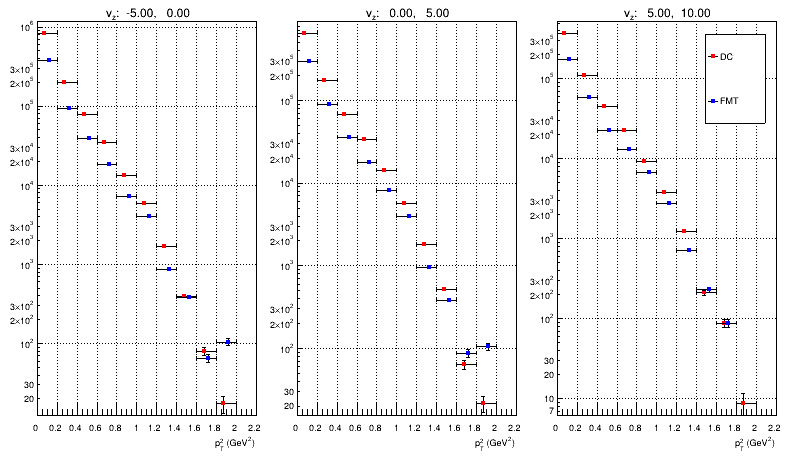
\includegraphics[width=\textwidth]{15pt2_pi+.png}}
                }
                \scriptsize{\textit{$p_T^2$ distributions for \ef{$\pi^+$}.}}
            \end{figure}
        \end{center}
    \end{column}

    \begin{column}{.54\linewidth}
        \begin{itemize}
            \item
                Large statistical fluctuations are observed for $p_T^2 > 1.4 \text{ GeV}^2$, as was expected.

            \vspace{12pt}
            \item
                \ef{No new restrictions on $v_z$ are derived from $p_T^2$.}
        \end{itemize}

        \vspace{109pt}

        \begin{flushright}
            \tiny{\textit{Bin markers are slightly shifted in $x$ for legibility.}}

            \vspace{-0.5pt}

            \tiny{\textit{
                Other bins can be seen in Slides \textcolor{efd_purple}{\ref{20.11e::pt2_pi+}} and \textcolor{efd_purple}{\ref{20.11f::pt2_pi-}}.
                Uncorrected bins in Slides \textcolor{efd_purple}{\ref{20.10e::pt2_pi+}} and \textcolor{efd_purple}{\ref{20.10f::pt2_pi-}}.
            }}
        \end{flushright}
    \end{column}

    \end{columns}
\end{frame}

% --+ 12.16 PHIPQ +-------------------------------------------------------------
\begin{frame}{Phase Space Study: $\phi_{PQ}$}
    \label{12.16::phipq}

    \begin{columns}[onlytextwidth,T]

    \begin{column}{.44\linewidth}
        \vspace{-15pt}
        \begin{center}
            \begin{figure}[t]
                \centering{
                    \fbox{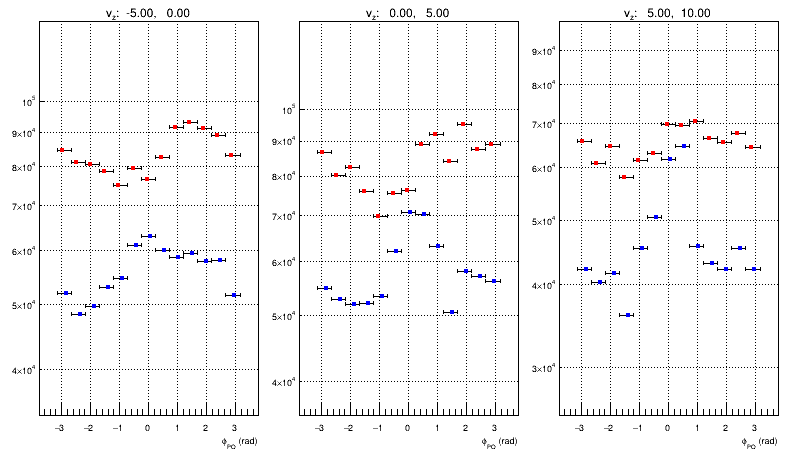
\includegraphics[width=\textwidth]{16phipq_pi-.png}}
                }
                \scriptsize{\textit{$\phi_{PQ}$ distributions for \ef{$\pi^-$}.}}
            \end{figure}

            \vspace{-15pt}
            \begin{figure}[t]
                \centering{
                    \fbox{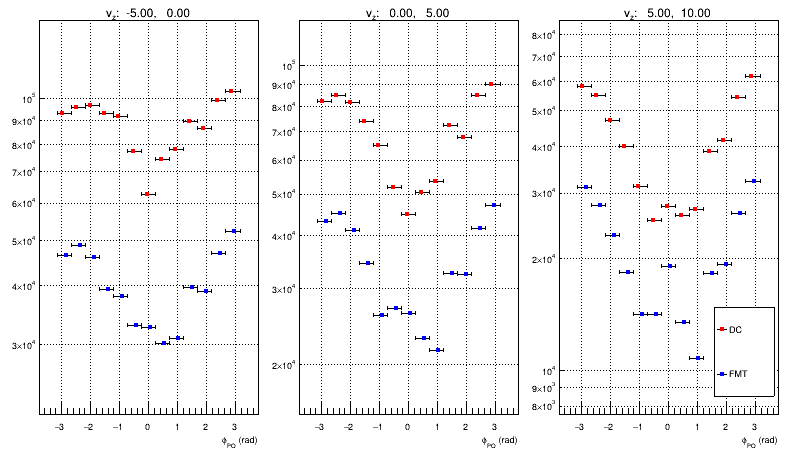
\includegraphics[width=\textwidth]{16phipq_pi+.png}}
                }
                \scriptsize{\textit{$\phi_{PQ}$ distributions for \ef{$\pi^+$}.}}
            \end{figure}
        \end{center}
    \end{column}

    \begin{column}{.54\linewidth}
        \begin{itemize}
            \item
                A shape analysis would be required to obtain conclusions from $\phi_{PQ}$.

            \vspace{12pt}
            \item
                % Considering the information already extracted from other variables,
                This is deemed unnecessary, and \ef{no new restrictions are obtained from $\phi_{PQ}$}.
        \end{itemize}

        \vspace{123pt}

        \begin{flushright}
            \tiny{\textit{Bin markers are slightly shifted in $x$ for legibility.}}

            \tiny{\textit{
                Other bins can be seen in Slides \textcolor{efd_purple}{\ref{20.11g::phipq_pi+}} and \textcolor{efd_purple}{\ref{20.11h::phipq_pi-}}.
                Uncorrected bins in Slides \textcolor{efd_purple}{\ref{20.10g::phipq_pi+}} and \textcolor{efd_purple}{\ref{20.10h::phipq_pi-}}.
            }}
        \end{flushright}
    \end{column}

    \end{columns}
\end{frame}


\subsection{Statistic Study}
% TODO. STATISTICS STUDY.

\subsection{Conclusions}
% TODO. CONCLUSIONS.
